% IEEEtran Conference Template for ECA-RAG
% Target: IEEE Conference Submission (8 pages)
\documentclass[conference]{IEEEtran}

\IEEEoverridecommandlockouts

% --- Packages ---
\usepackage{amsmath,amssymb,amsfonts}
\usepackage{algorithmic}
\usepackage{graphicx}
\usepackage{textcomp}
\usepackage{xcolor}
\usepackage{booktabs}
\usepackage{cite}
\usepackage{url}
\usepackage{multirow}
\usepackage{microtype}
\usepackage{balance}

\def\BibTeX{{\rm B\kern-.05em{\sc i\kern-.025em b}\kern-.08em
    T\kern-.1667em\lower.7ex\hbox{E}\kern-.125emX}}

\begin{document}

% =========================================================================
% TITLE & AUTHORS
% TODO: working title, confirm with guide
% =========================================================================
\title{ECA-RAG: Calibrated Confidence, Hop-Conditioned Re-Ranking, and the Limits of Adaptive-$k$ Retrieval in Multi-Hop RAG}

\author{
    \IEEEauthorblockN{Jaiyandh Amutha Sugumar\IEEEauthorrefmark{1}, Adwaith Murali\IEEEauthorrefmark{2}, Ariya Kumar\IEEEauthorrefmark{3}}
    \IEEEauthorblockA{
        \textit{Department of Computer Science and Engineering}\\
        \textit{Kongu Engineering College}\\
        Perundurai, Erode, Tamil Nadu, India\\
        Email: \IEEEauthorrefmark{1}jaiyandh@gmail.com, \IEEEauthorrefmark{2}adwaithmurali2005@gmail.com, \IEEEauthorrefmark{3}ariyakumar258@gmail.com
    }
}

\maketitle

% =========================================================================
% ABSTRACT (Strictly <= 200 words; currently 193 words)
% =========================================================================
\begin{abstract}
Adaptive retrieval-augmented generation (RAG) dynamically adjusts retrieval depth $k$ to balance sufficiency against compute. We evaluate calibrated confidence and iterative adaptive-$k$ retrieval on HotpotQA ($N=2640$ matched-depth). First, cross-encoder logits are miscalibrated; Platt scaling reduces Expected Calibration Error from 0.225 to 0.039 and Brier score from 0.213 to 0.116 on 5,385 held-out eval chunk predictions ($N=540$). Second, gating on calibrated scores does not beat fixed-$k$ at matched depth $k=4.00$: calibrated single-pass gating underperforms fixed-$k$ by 2.7 points ($\Delta = -0.027$, Holm $p < 0.001$), while iterative gated retrieval does not differ significantly from fixed-$k$ ($\Delta = -0.0088$, raw $p=0.079$, Holm $p=0.079$), costing 2.6 points relative to ungated iteration ($\Delta = -0.0257$, Holm $p < 0.001$). Third, hop-conditioned reformulation yields modest bridge gains ($+1.7$ points, $\Delta = +0.017$, Holm $p=0.001$) while degrading comparison queries ($-2.4$ points, $\Delta = -0.024$, Holm $p=0.007$). Finally, in exploratory multi-depth analysis, a learned sufficiency stopper (ROC AUC 0.80) performs comparably to fixed-$k$ on bridge questions across $k \in [2.0, 3.5]$, but is significantly worse on comparison queries ($\Delta = -0.138$ to $-0.044$, all Holm $p < 0.001$), while improving upon iterative gating on both types (all Holm $p < 0.001$).
\end{abstract}

\begin{IEEEkeywords}
Retrieval-Augmented Generation, Multi-Hop Question Answering, Confidence Calibration, Adaptive Retrieval, Cross-Encoder Re-Ranking.
\end{IEEEkeywords}

% =========================================================================
% I. INTRODUCTION
% =========================================================================
\section{Introduction}
\label{sec:intro}
To mitigate factual hallucinations and supply up-to-date knowledge, Retrieval-Augmented Generation (RAG) pairs Large Language Models (LLMs) with external reference collections during prompt construction~\cite{collini2025carag,asai2024selfrag}. However, typical RAG pipelines employ a static retrieval depth, retrieving a fixed number of context chunks ($k$) for every user query regardless of query complexity~\cite{kratzwald2018adaptive,jeong2024adaptiverag}. In multi-hop reasoning tasks—where answering a question requires finding and synthesizing disjoint supporting facts across multiple documents~\cite{yang2018hotpotqa}—fixed-$k$ retrieval presents a direct trade-off: small values of $k$ risk omitting necessary reasoning steps (under-retrieval), while larger values introduce irrelevant text that degrades reader precision and increases computational cost (over-retrieval).

Recent investigations attempt to overcome this rigid trade-off by dynamically tuning retrieval depth or query invocation on the fly~\cite{kratzwald2018adaptive,jeong2024adaptiverag,wang2024targ,liu2024ctrla}. A common approach is confidence-based gating, which filters candidate passages using relevance scores from retrieval or re-ranking models~\cite{collini2025carag}. However, modern deep neural networks and transformer cross-encoders are known to be miscalibrated, frequently producing overconfident predictions~\cite{guo2017calibration}. Uncalibrated raw scores cannot be directly interpreted as true probabilities of relevance, making heuristic score thresholds sensitive to distribution shifts across query types.

In this work, we investigate the empirical interaction of post-hoc probability calibration, hop-conditioned re-ranking, and adaptive-$k$ stopping policies in multi-hop RAG. We evaluate six retrieval configurations on the HotpotQA benchmark~\cite{yang2018hotpotqa}, scaling the evaluation across an initial calibration and evaluation split to an extended pooled sample of $N=2640$ question--context instances.

Because adaptive stopping policies alter both the average context depth ($k$) and retrieval recall concurrently, unconstrained evaluations risk confounding the stopping heuristic with the simple baseline benefit of reading more text chunks. To cleanly isolate algorithmic selection from raw passage volume, we enforce strict matched-depth comparisons at average depth $k=4.00$, complemented by an exploratory evaluation over target depths $k \in \{2.0, 2.5, 3.0, 3.5, 4.0, 4.5, 5.0, 5.5\}$ using 10,000 paired bootstrap resamples.

Our primary empirical findings are:
\begin{enumerate}
    \item \textbf{Calibration Quality:} Raw cross-encoder relevance logits exhibit substantial miscalibration on the held-out $N=540$ evaluation split ($\text{ECE}=0.2248$, Brier score $0.2127$, evaluated over the exact 5,385 candidate chunk predictions from the 540-example held-out split, not the $N=2640$ pool). Chunk-level Platt scaling~\cite{platt1999probabilistic} reduces ECE by 82.6\% to $0.0391$ and cuts Brier score to $0.1157$.
    \item \textbf{Limits of Calibrated Gating at $k=4.00$:} Gating retrieval on calibrated chunk probabilities does not exceed static fixed-$k$ baselines at matched depth $k=4.00$. Calibrated single-pass gating underperforms fixed-$k$ re-ranking by $2.7$ points recall on bridge questions ($\Delta = -0.0266$, $95\%$ CI $[-0.0341, -0.0191]$, Holm $p < 0.001$). Iterative gated retrieval yields recall statistically indistinguishable from fixed-$k$ on bridge questions ($\Delta = -0.0088$, $95\%$ CI $[-0.0187, +0.0010]$, raw $p=0.0794$, Holm $p=0.0794$ within the 5-contrast bridge family at $k=4.00$, $95\%$ CI includes zero), but costs $2.6$ points recall relative to ungated iteration ($\Delta = -0.0257$, $95\%$ CI $[-0.0328, -0.0186]$, Holm $p < 0.001$).
    \item \textbf{Asymmetric Multi-Hop Reformulation:} Hop-conditioned query reformulation at fixed depth $k=4.00$ yields a modest, statistically significant gain on bridge questions ($+1.7$ points, $\Delta = +0.017$, $95\%$ CI $[+0.0077, +0.0258]$, Holm $p=0.001$), but degrades comparison questions ($-2.4$ points, $\Delta = -0.024$, $95\%$ CI $[-0.0391, -0.0089]$, Holm $p=0.007$).
    \item \textbf{Depth-Dependent Trajectories and Sufficiency Stopping:} In exploratory multi-depth analysis, iterative gating lags behind fixed-$k$ at tight budgets ($k \le 3.5$, all Holm $p \le 0.005$) and converges with fixed-$k$ from $k=4.0$ to $k=5.0$. At $k=5.5$, it attains an exploratory $+0.0127$ recall ($95\%$ CI $[+0.0044, +0.0210]$, Holm $p=0.0176$). A learned sufficiency stopping classifier (ROC AUC $0.7964$) remains statistically indistinguishable from fixed-$k$ on bridge questions across all covered depths ($k \in [2.0, 3.5]$, with 95\% CIs spanning zero). However, on comparison questions, the stopper is significantly worse than fixed-$k$ at every covered depth $k \in [2.0, 3.5]$ ($\Delta = -0.138$ to $-0.044$, all Holm $p < 0.001$). Nonetheless, in exploratory analysis it improves upon iterative gating (Arm 5) on both question types at $k \in [2.0, 3.5]$ ($+1.5$ to $+5.3$ points on bridge, $+3.4$ to $+5.5$ points on comparison, all Holm $p < 0.001$).
\end{enumerate}

% =========================================================================
% II. RELATED WORK
% =========================================================================
\section{Related Work}
\label{sec:related}

\subsection{Context-Aware and Re-Ranked RAG}
Standard dense retrieval models employ bi-encoder architectures that map queries and documents into a shared vector space independently, enabling fast approximate nearest neighbor search but sacrificing token-level cross-attention. Cross-encoder re-rankers improve precision by processing concatenated query--document text. Collini et al.~\cite{collini2025carag} introduced Context-Aware RAG (CA-RAG), demonstrating that filtering context inconsistencies via similarity validation improves generation faithfulness. In our framework, Arm 1 serves as a CA-RAG-style dense retrieval baseline, over which we evaluate cross-encoder re-ranking, post-hoc calibration, and multi-hop gating.

\subsection{Adaptive and Dynamic Retrieval}
Adaptive retrieval approaches adjust retrieval depth or frequency based on query characteristics. Kratzwald and Feuerriegel~\cite{kratzwald2018adaptive} investigated query-adaptive document retrieval depths for deep question answering. Adaptive-RAG~\cite{jeong2024adaptiverag} routes queries to no-retrieval, single-step, or multi-step paths via a complexity classifier. Training-free gating methods, such as TARG~\cite{wang2024targ} (which decides retrieval necessity via draft-token entropy and logit margin) and CtrlA~\cite{liu2024ctrla} (which steers retrieval through honesty and confidence directions in LLM internal representations), assess when retrieval is required. For long-form text generation, active methods such as FLARE~\cite{jiang2023flare}, Self-RAG~\cite{asai2024selfrag}, and DRAGIN~\cite{su2024dragin} dynamically trigger retrieval when confidence falls below fixed thresholds. However, these systems focus primarily on retrieval invocation rather than resolving the optimal chunk count ($k$) under matched-depth constraints.

\subsection{Confidence Calibration in Neural Systems}
Guo et al.~\cite{guo2017calibration} showed that modern neural networks often output uncalibrated probabilities that overestimate empirical correctness. Post-processing methods such as temperature scaling and Platt scaling~\cite{platt1999probabilistic} fit parametric mappings on held-out validation sets to convert raw scores into calibrated posterior probabilities. We examine whether recalibrating cross-encoder relevance logits can support robust stopping thresholds in multi-hop retrieval.

\subsection{Multi-Hop Retrieval Architectures}
Multi-hop question answering requires traversing reasoning chains across disconnected documents. Multi-hop Dense Retrieval (MDR)~\cite{xiong2021mdr} and Baleen~\cite{khattab2021baleen} train specialized multi-hop encoders to navigate document graphs. Interleaved methods like IRCoT~\cite{trivedi2023ircot} interleave chain-of-thought generation with retrieval hops. In contrast to training specialized multi-hop encoders, we examine whether post-hoc calibration and confidence gating can govern retrieval depth using off-the-shelf bi-encoder and cross-encoder models.

% =========================================================================
% III. METHODOLOGY & EXPERIMENTAL FRAMEWORK
% =========================================================================
\section{Methodology}
\label{sec:method}

\subsection{System Architecture and Evaluation Arms}
We evaluate six retrieval paradigms (Arms 1--6) operating over the per-question pool of $\sim 10$ paragraphs in HotpotQA's distractor setting:
\begin{itemize}
    \item \textbf{Arm 1 (Dense Baseline):} Encodes query $q$ and retrieves the top-$k$ passages ranked by cosine similarity using a bi-encoder: $\mathcal{D}_1 = \text{Top-}k_{d \in \mathcal{P}} \langle \mathbf{e}_q, \mathbf{e}_d \rangle$, where $\mathcal{P}$ is the per-question candidate pool.
    \item \textbf{Arm 2 (Fixed-$k$ Cross-Encoder):} Retrieves an initial candidate pool of $M=10$ passages using Arm 1, then computes full cross-attention relevance logits $s(q, d)$ with a cross-encoder (truncated to 512 tokens). Passages are selected under fixed integer cutoffs $k \in \{1, 2, 3, 4, 5, 6\}$.
    \item \textbf{Arm 3 (Uncalibrated Marginal Gating):} Walks down the ranked candidate list from the cross-encoder, selecting passages where raw score $s(q, d) \ge s_{\text{thresh}}$, with a minimum of 1 and a maximum of 6 chunks.
    \item \textbf{Arm 4 (Calibrated Single-Pass Gating):} Transforms raw logits $s$ into calibrated probabilities $\hat{p} = \sigma(a \cdot s + b)$ via Platt scaling and walks down the ranked list, selecting passages satisfying $\hat{p} \ge \theta$, with a minimum of 1 and a maximum of 6 chunks. We evaluate both global pooled scaling (\textbf{Arm 4a}) and question-type-conditioned parameters (\textbf{Arm 4b}).
    \item \textbf{Arm 5 (Calibrated Iterative Adaptive-$k$):} Iterates up to 6 hops over the per-question candidate pool. At hop 0, remaining candidates are scored against query $q$ alone; at each subsequent hop $h \ge 1$, the cross-encoder scores all remaining candidates against $q$ concatenated with the full text of the previously selected chunk ($q \oplus \text{ `` ''} \oplus d_{(h)}$). The best candidate is selected; for hops $h \ge 1$, retrieval stops if its per-type Platt probability falls below $\theta$ (max 6 chunks). No bi-encoder is used after the initial candidate pool is formed; 50-word truncation is evaluated only as an ablation in Section~\ref{sec:results-ablation}.
    \item \textbf{Arm 6 (Learned Sufficiency Stopping):} Evaluates a supervised logistic regression classifier with feature standardization trained on calibration traces. The classifier uses 6 features: calibrated probability of the next candidate, its raw cross-encoder score, hop index, probability drop from the previous hop, minimum calibrated probability among already selected chunks, and a binary indicator for bridge questions (\texttt{is\_bridge}). The binary training label indicates whether all gold supporting paragraphs have already been selected. At each hop $h \ge 1$, retrieval stops if candidate probability falls below $\theta$ or if posterior $P(\text{sufficient} \mid \mathbf{x}) \ge \tau$ (subject to a 6-chunk ceiling).
\end{itemize}

\subsection{Chunk-Level Platt Calibration}
Given a cross-encoder scoring query--passage pairs $(q, d) \to s \in \mathbb{R}$, we fit an affine transformation mapped through the logistic sigmoid function~\cite{platt1999probabilistic}:
\begin{equation}
    P(y = 1 \mid s) = \sigma(a \cdot s + b) = \frac{1}{1 + \exp(-(a \cdot s + b))}
\end{equation}
where $y \in \{0, 1\}$ denotes binary ground-truth supporting paragraph relevance. Parameters $a, b \in \mathbb{R}$ are estimated on the calibration split by minimizing binary cross-entropy:
\begin{equation}
    \mathcal{L}(a, b) = -\sum_{i=1}^{N_{\text{cal}}} \left[ y_i \log \hat{p}_i + (1 - y_i) \log(1 - \hat{p}_i) \right]
\end{equation}
Calibration quality is evaluated using Expected Calibration Error (ECE) across $M=10$ equal-width probability bins $B_m \subset (0, 1]$:
\begin{equation}
    \text{ECE} = \sum_{m=1}^M \frac{|B_m|}{N} \left| \text{acc}(B_m) - \text{conf}(B_m) \right|
\end{equation}
alongside the Brier score: $\text{BS} = \frac{1}{N}\sum_{i=1}^N (\hat{p}_i - y_i)^2$.

\subsection{Hop-Conditioned Iterative Re-Ranking}
For multi-hop questions, early retrieval hops often surface an introductory entity whose text reveals intermediate entities required for subsequent reasoning. In Arm 5 and ungated iterative retrieval, retrieval iterates up to 6 hops over the per-question pool of $\sim 10$ candidate paragraphs without re-invoking the bi-encoder. At hop 0, candidate passages are scored against $q$ alone. At each subsequent hop $h \ge 1$, the cross-encoder scores all remaining candidates against the question concatenated with the full text of the chunk selected at hop $h-1$:
\begin{equation}
    q^{(h+1)} = q \oplus \text{ `` ''} \oplus d_{(h)}
\end{equation}
The highest-scoring remaining passage is selected. In Arm 5, for hops $h \ge 1$, retrieval terminates if the candidate's per-type Platt probability falls below threshold $\theta$ (min 1, max 6 chunks). In Section~\ref{sec:results-ablation}, we ablate this full-chunk concatenation against a 50-word prefix truncation variant ($q \oplus \text{ `` ''} \oplus \text{Trunc}_{50}(d_{(h)})$) to evaluate whether passage length introduces token dilution during cross-encoder re-ranking.

\subsection{Reproducibility Protocol and Frozen Parameters}
To ensure reproducibility:
\begin{itemize}
    \item \textbf{Dataset and Splits:} We use the HotpotQA validation set in the distractor setting ($N=3000$ total examples drawn from the full validation set of 7,405 examples, each paired with a candidate pool of $\sim 10$ paragraphs)~\cite{yang2018hotpotqa}. The 3,000 examples are the first 3,000 of the seed-42 shuffled HotpotQA distractor validation set. A seed-42 random split partitioned the first 900 example IDs into the first 40\% ($N=360$; 279 bridge, 81 comparison) for calibration and the remaining 60\% ($N=540$; 424 bridge, 116 comparison) for held-out evaluation (these are not contiguous index slices of the unshuffled dataset). The extension split ($N=2100$; 1653 bridge, 447 comparison) comprises elements 900 to 2999 from the same seed-42 shuffled HotpotQA distractor validation set; its example IDs are verified to be strictly disjoint from the first 900 examples. The pooled dataset ($N=2640$; 2077 bridge, 563 comparison) concatenates the evaluation and extension splits.
    \item \textbf{Models and Versions:} Dense retrieval uses \texttt{sentence-transformers/all-MiniLM-L6-v2} (384-dimensional embeddings, cosine similarity). Cross-encoder re-ranking uses \texttt{cross-encoder/ms-marco-MiniLM-L-6-v2} with a 512-token truncation limit.
    \item \textbf{Frozen Calibration Parameters:} Parameters fit on the $N=360$ calibration split are held frozen across all evaluation splits:
    \begin{itemize}
        \item Platt parameters: Pooled ($a=0.2703, b=-1.3639$); Bridge ($a=0.2454, b=-1.3621$); Comparison ($a=0.4724, b=-1.4665$).
        \item Confidence threshold: $\theta^* = 0.18$ was selected on the calibration split to maximize recall subject to mean depth $k \le 4.0$. Sensitivity is evaluated at $\theta = 0.15$.
        \item Uncalibrated threshold: $s_{\text{thresh}} = -1.9250$ (median logit on calibration split).
        \item Sufficiency stopper: $\tau^* = 0.95$ (tuned on calibration traces).
    \end{itemize}
    \item \textbf{Random Seed:} All data partitioning and bootstrap iterations use seed 42.
\end{itemize}

% =========================================================================
% IV. EMPIRICAL EVALUATION & RESULTS
% =========================================================================
\section{Empirical Evaluation and Results}
\label{sec:results}

% --- TABLE I: CALIBRATION QUALITY ---
\begin{table}[t]
\centering
\caption{Cross-Encoder Calibration Quality on $N=540$ Evaluation Split (5,385 Candidate Chunk Predictions)}
\label{tab:calibration}
\begin{tabular}{lccc}
\toprule
\textbf{Calibration Method} & \textbf{ECE} $\downarrow$ & \textbf{Brier Score} $\downarrow$ & \textbf{ECE Red.} \\
\midrule
Raw Sigmoid $\sigma(s)$ & 0.2248 & 0.2127 & Baseline \\
Platt Scaling (Pooled)  & 0.0419 & 0.1161 & 81.4\% \\
Platt Scaling (Per-Type) & \textbf{0.0391} & \textbf{0.1157} & \textbf{82.6\%} \\
\bottomrule
\end{tabular}
\end{table}

\subsection{Calibration Quality}
Table~\ref{tab:calibration} reports calibration metrics for raw versus Platt-scaled cross-encoder logits on the held-out $N=540$ evaluation set (exact 5,385 candidate chunk predictions, not the pooled $N=2640$ cohort). Raw logits mapped through a standard sigmoid display high miscalibration ($\text{ECE}=0.2248$, Brier score $0.2127$), overestimating the probability of relevance for negative distractor paragraphs.

Platt scaling reduces ECE to $0.0419$ (pooled) and $0.0391$ (per-type), achieving an $82.6\%$ relative reduction in calibration error. The Brier score drops by $45.6\%$ to $0.1157$. Conditioning calibration on question type provides a minor gain, reflecting slightly different logit distributions between bridge and comparison queries. Platt parameters transferred robustly to the $N=2100$ extension split (20,901 candidate chunk predictions): raw logits exhibited $\text{ECE}=0.2143$ and Brier score $0.2039$, whereas frozen per-type Platt scaling achieved $\text{ECE}=0.0373$ (an $82.6\%$ relative reduction) and Brier score $0.1146$ (pooled Platt: $\text{ECE}=0.0389$, Brier score $0.1162$), demonstrating that the calibration parameters generalize stably across independent question sets.

% --- TABLE II: HEADLINE MATCHED DEPTH (POOLED N=2640) ---
\begin{table*}[t]
\centering
\caption{Matched-Depth Paragraph Recall at Exact Mean Depth $k=4.00$ Across Evaluation Cohorts}
\label{tab:matched_depth}
\resizebox{\textwidth}{!}{%
\begin{tabular}{llccccc}
\toprule
\textbf{Split / Dataset} & \textbf{Type ($N$)} & \textbf{Fixed-$k$ ($k=4$)} & \textbf{Iterative ($k=4$, No Gate)} & \textbf{Arm 5 (Interp. $k=4$)} & \textbf{Arm 4b (Interp. $k=4$)} & \textbf{Arm 6 (Interp. $k=4$)} \\
\midrule
\multirow{2}{*}{$N=540$ Component Split} 
 & Bridge (424)     & 0.8054 & 0.8160 & 0.8013 & 0.7693 & n/a \\
 & Comparison (116) & \textbf{0.9483} & 0.9181 & 0.8649 & 0.9479 & 0.8712$^*$ \\
\midrule
\multirow{2}{*}{$N=2100$ Component Split} 
 & Bridge (1653)     & 0.8076 & \textbf{0.8261} & 0.7978 & 0.7835 & n/a \\
 & Comparison (447)  & \textbf{0.9553} & 0.9329 & 0.9273 & 0.9530 & 0.9280$^*$ \\
\midrule
\multirow{2}{*}{\textbf{Pooled Headline ($N=2640$)}} 
 & \textbf{Bridge (2077)}     & 0.8072 & \textbf{0.8240} & 0.7983 & 0.7806 & n/a \\
 & \textbf{Comparison (563)} & \textbf{0.9538} & 0.9298 & 0.9147 & 0.9520 & 0.9168$^*$ \\
\bottomrule
\end{tabular}%
}
\vspace{1ex}
\begin{flushleft}
\footnotesize \textit{Note on Linear Interpolation and Arm 6:} To ensure rigorous comparisons at matched retrieval depth $k=4.00$, points for Arm 5 and Arm 4b are evaluated via piece-wise linear interpolation between empirical sweep points. For Arm 5 on bridge, the bracketing points are $\theta=0.18$ ($k=3.8671$, recall $0.7913$) and $\theta=0.16$ ($k=4.2297$, recall $0.8105$), linearly interpolating to recall $0.7983$ at $k=4.0000$. Arm 6 values on bridge are reported as n/a because early sufficiency stopping caps its maximum depth near $k=3.87$ under frozen calibration threshold $\theta^*=0.18$, so it never reaches depth $k=4.00$. On comparison questions, Arm 6 attains mean depths up to $k \approx 4.04\text{--}4.20$, producing point estimates of $0.8712$ ($N=540$), $0.9280$ ($N=2100$), and $0.9168$ (Pooled, marked $^*$). However, because under 95\% of paired bootstrap draws achieve $k=4.00$, non-parametric hypothesis tests and confidence intervals cannot be reliably computed at this depth.
\end{flushleft}
\end{table*}

\subsection{Matched-Depth Evaluation at Reference Depth $k=4.00$}
Table~\ref{tab:matched_depth} presents our matched-depth results at exact mean depth $k=4.00$, comparing static fixed-$k$ retrieval against ungated iterative retrieval and calibrated adaptive gating across the pooled $N=2640$ cohort as well as the constituent $N=540$ and $N=2100$ splits.

\subsubsection{Bridge Questions}
On the pooled bridge cohort ($N=2077$), ungated iterative retrieval attains a recall of $0.8240$, compared to $0.8072$ for fixed-$k$ retrieval ($\Delta = +0.0169$, $95\%$ CI $[+0.0077, +0.0258]$, $p < 0.001$, Holm $p=0.001$). Gating retrieval on calibrated scores does not improve recall over fixed-$k$: Arm 5 attains an interpolated recall of $0.7983$, displaying no statistically significant divergence from fixed-$k$ ($\Delta = -0.0088$, $95\%$ CI $[-0.0187, +0.0010]$, raw $p = 0.0794$, Holm $p = 0.0794$).

Relative to ungated iteration at identical depth, gating incurs a recall cost of $2.6$ points ($\Delta = -0.0257$, $95\%$ CI $[-0.0328, -0.0186]$, $p < 0.001$, Holm $p < 0.001$). Calibrated single-pass gating (Arm 4b) performs significantly below fixed-$k$ at matched depth, reaching $0.7806$ recall ($\Delta = -0.0266$, $95\%$ CI $[-0.0341, -0.0191]$, $p < 0.001$).

\subsubsection{Comparison Questions}
On the pooled comparison cohort ($N=563$), static fixed-$k$ retrieval attains $0.9538$ recall. Ungated iterative search attains a lower recall of $0.9298$ ($\Delta = -0.0240$, $95\%$ CI $[-0.0391, -0.0089]$, $p = 0.002$, Holm $p=0.007$). Arm 4b calibrated single-pass gating achieves $0.9520$ recall, which is indistinguishable from fixed-$k$ ($\Delta = -0.0018$, $95\%$ CI $[-0.0136, +0.0095]$, raw $p = 0.7202$, Holm $p = 0.7202$). Iterative gated retrieval (Arm 5) reaches $0.9147$ ($\Delta = -0.0391$, $95\%$ CI $[-0.0565, -0.0221]$, $p < 0.001$).

% --- FIGURE 1: PARETO EFFICIENCY-RECALL CURVES ---
\begin{figure*}[t]
\centering
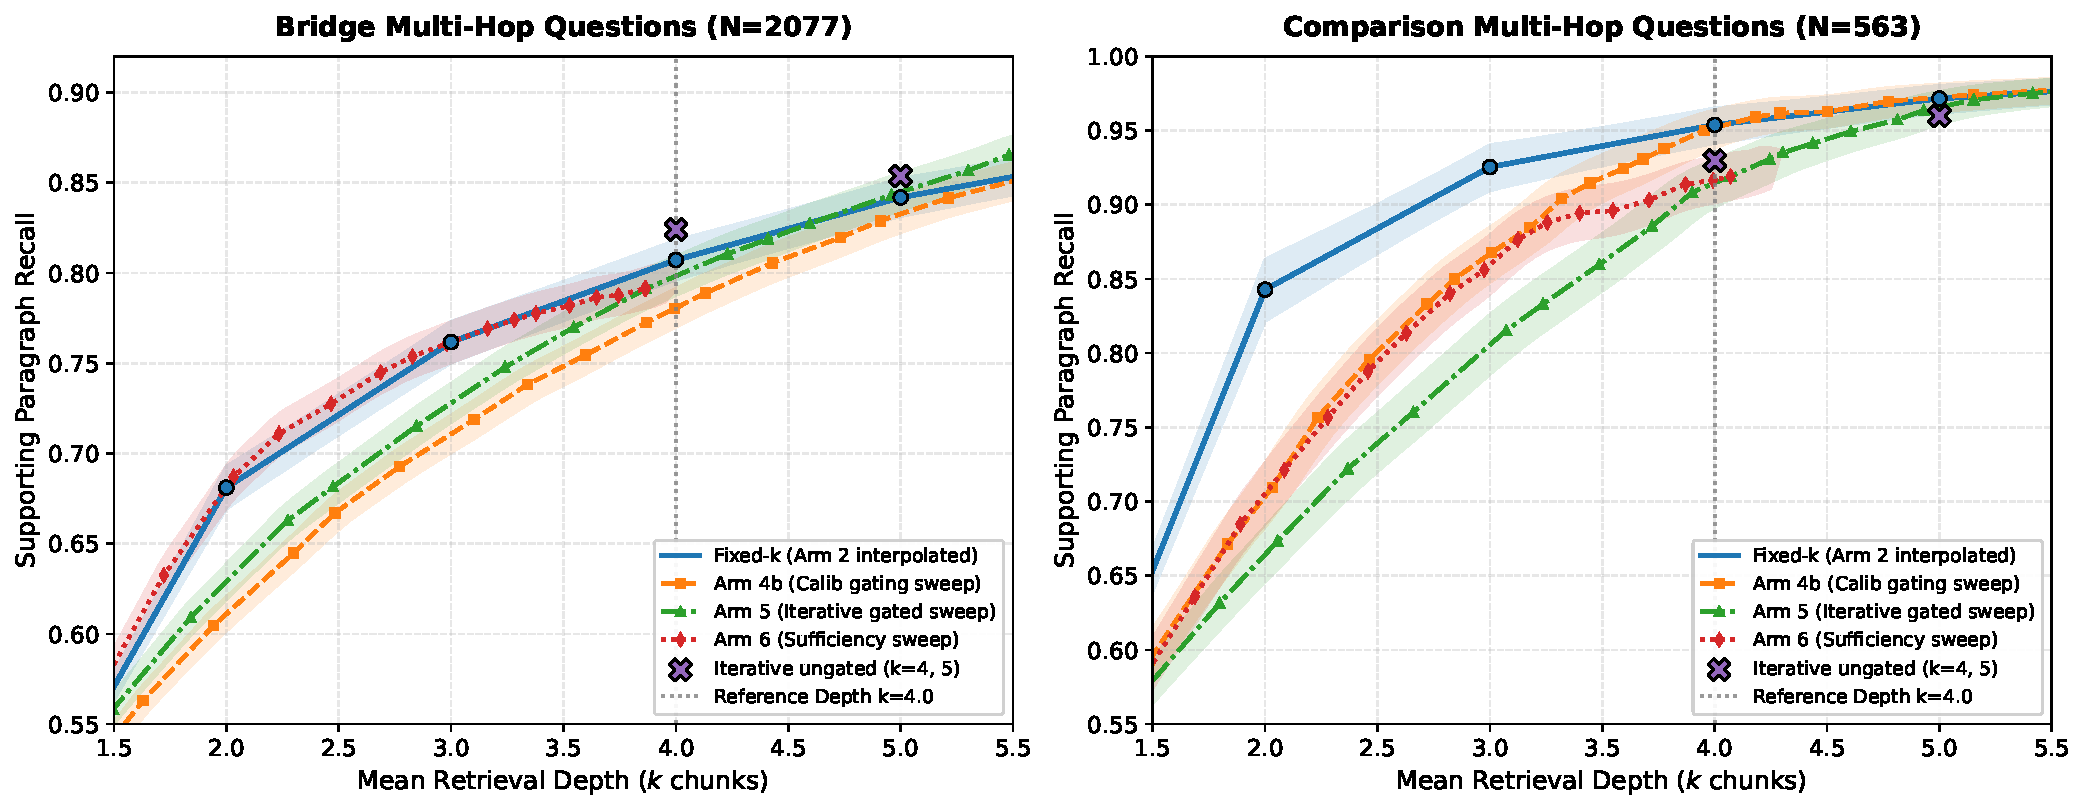
\includegraphics[width=0.96\textwidth]{figures/fig_pareto_recall_vs_k.pdf}
\caption{Recall--efficiency Pareto frontiers across mean retrieval depth ($k$) on pooled HotpotQA validation questions ($N=2640$; bridge $N=2077$, comparison $N=563$, pooled from the 540 held-out evaluation and 2100 extension splits). Solid blue curve denotes static Fixed-$k$ retrieval (Arm 2), where the continuous line represents the linear mixture of $\lfloor k \rfloor$ and $\lceil k \rceil$, an achievable time-sharing baseline rather than a smoothing artifact, with discrete markers at integer depths $k \in \{1, 2, 3, 4, 5, 6\}$. Dashed orange curve represents Calibrated Single-Pass Gating (Arm 4b, swept over $\theta$). Dash-dotted green curve represents Calibrated Iterative Gating (Arm 5, swept over $\theta$). Dotted red curve denotes Learned Sufficiency Stopping (Arm 6, swept over $\tau$ with $\theta^*=0.18$). On bridge questions Arm 6 does not reach $k \ge 4.0$ because its inner candidate threshold $\theta^*=0.18$ caps its maximum depth near $k=3.87$; on comparison it reaches $k$ of about 4.04--4.20. Shaded ribbons represent pointwise 95\% paired bootstrap confidence bands across $B=10{,}000$ resamples (not simultaneous confidence bands; overlapping bands do not imply lack of statistical significance, as paired differences in Table V are tighter). Purple markers indicate Ungated Iterative retrieval at fixed depths $k=4$ and $k=5$. The vertical dotted line marks the $k=4.0$ reference operating budget. Both panels use a common y-axis lower limit of 0.55 for direct visual comparability.}
\label{fig:pareto}
\end{figure*}

\subsection{Pareto Frontiers of Retrieval Efficiency}
Fig.~\ref{fig:pareto} shows the empirical Pareto frontiers of Paragraph Recall versus Mean Retrieval Depth ($k$) across bridge and comparison subsets on the pooled $N=2640$ dataset, displaying pointwise 95\% bootstrap confidence bands ($B=10{,}000$).
\begin{itemize}
    \item \textbf{Bridge Structure:} The fixed-$k$ curve traces a concave frontier across retrieval depths ($0.6810$ at $k=2.0$ to $0.8533$ at $k=5.5$). Calibrated single-pass gating (Arm 4b) lies below the fixed-$k$ envelope through $k=5.0$. Iterative gating (Arm 5) shifts the adaptive frontier upward, converging with fixed-$k$ at $k \ge 4.0$. At $k=4$, ungated iterative retrieval clears the fixed-$k$ curve, whereas at $k=5$ it sits marginally above it.
    \item \textbf{Comparison Structure:} The fixed-$k$ curve forms an upper envelope. All adaptive gating sweeps (Arm 4b, Arm 5, Arm 6) remain bounded by fixed-$k$. As gating becomes more aggressive (higher $\theta$ or $\tau$), recall falls faster than under static top-$k$ truncation.
\end{itemize}

% --- TABLE III: FULL RETRIEVAL BENCHMARK SPLITS ---
\begin{table*}[t]
\centering
\caption{Full Retrieval Performance Across Evaluation Splits ($N=540$ Eval and $N=2100$ Extension)}
\label{tab:full_eval}
\resizebox{\textwidth}{!}{%
\begin{tabular}{llcccccccc}
\toprule
& & \multicolumn{4}{c}{\textbf{Initial Eval Split ($N=540$)}} & \multicolumn{4}{c}{\textbf{Extension Split ($N=2100$)}} \\
\cline{3-6} \cline{7-10}
\textbf{Method} & \textbf{Type} & \textbf{Recall} & \textbf{Precision} & \textbf{Full-Match} & \textbf{Mean $k$} & \textbf{Recall} & \textbf{Precision} & \textbf{Full-Match} & \textbf{Mean $k$} \\
\midrule
\multirow{2}{*}{Arm 1 (Dense Baseline $k=4$)}
 & Bridge     & 0.7559 & 0.3779 & 0.5354 & 4.000 & 0.7429 & 0.3728 & 0.5275 & 4.000 \\
 & Comparison & 0.9138 & 0.4569 & 0.8362 & 4.000 & 0.9306 & 0.4691 & 0.8613 & 4.000 \\
\midrule
\multirow{2}{*}{Arm 2 (Fixed-$k$ CE, $k=4$)}
 & Bridge     & 0.8054 & 0.4027 & 0.6132 & 4.000 & 0.8076 & 0.4051 & 0.6261 & 3.995 \\
 & Comparison & 0.9483 & 0.4741 & 0.8966 & 4.000 & 0.9553 & 0.4814 & 0.9128 & 3.984 \\
\midrule
\multirow{2}{*}{Arm 2 (Fixed-$k$ CE, $k=5$)}
 & Bridge     & 0.8314 & 0.3328 & 0.6627 & 4.998 & 0.8445 & 0.3394 & 0.6975 & 4.992 \\
 & Comparison & 0.9698 & 0.3879 & 0.9397 & 5.000 & 0.9720 & 0.3939 & 0.9441 & 4.971 \\
\midrule
\multirow{2}{*}{Arm 3 (Uncalib. Gating, $s \ge -1.925$)}
 & Bridge     & 0.7818 & 0.4895 & 0.5684 & 4.158 & --- & --- & --- & --- \\
 & Comparison & 0.9612 & 0.4983 & 0.9224 & 4.534 & --- & --- & --- & --- \\
\midrule
\multirow{2}{*}{Arm 4a (Calib. Gating, $\theta^*=0.18$)}
 & Bridge     & 0.7394 & 0.5670 & 0.4858 & 3.535 & --- & --- & --- & --- \\
 & Comparison & 0.9353 & 0.6046 & 0.8793 & 3.845 & --- & --- & --- & --- \\
\midrule
\multirow{2}{*}{Arm 4b (Calib. Gating, $\theta^*=0.18$)}
 & Bridge     & 0.7417 & 0.5581 & 0.4906 & 3.594 & 0.7577 & 0.5659 & 0.5227 & 3.598 \\
 & Comparison & 0.9224 & 0.6345 & 0.8534 & 3.629 & 0.9128 & 0.6673 & 0.8277 & 3.398 \\
\midrule
\multirow{2}{*}{Arm 4b (Sensitivity, $\theta=0.15$)}
 & Bridge     & 0.7677 & 0.5113 & 0.5401 & 3.976 & 0.7834 & 0.5148 & 0.5729 & 3.998 \\
 & Comparison & 0.9353 & 0.6046 & 0.8793 & 3.845 & 0.9295 & 0.6358 & 0.8613 & 3.640 \\
\midrule
\multirow{2}{*}{Arm 5 (Iter. Gated, $\theta^*=0.18$)}
 & Bridge     & 0.7983 & 0.5107 & 0.6108 & 3.934 & 0.7895 & 0.5204 & 0.5935 & 3.850 \\
 & Comparison & 0.8793 & 0.4947 & 0.7759 & 4.198 & 0.9295 & 0.5559 & 0.8591 & 4.038 \\
\midrule
\multirow{2}{*}{Arm 5 (Sensitivity, $\theta=0.15$)}
 & Bridge     & 0.8243 & 0.4523 & 0.6604 & 4.455 & 0.8173 & 0.4582 & 0.6461 & 4.399 \\
 & Comparison & 0.9138 & 0.4701 & 0.8362 & 4.560 & 0.9407 & 0.5333 & 0.8814 & 4.237 \\
\midrule
\multirow{2}{*}{Iterative Ungated ($k=4$)}
 & Bridge     & 0.8160 & 0.4080 & 0.6462 & 4.000 & 0.8261 & 0.4143 & 0.6673 & 3.995 \\
 & Comparison & 0.9181 & 0.4591 & 0.8534 & 4.000 & 0.9329 & 0.4702 & 0.8658 & 3.984 \\
\midrule
\multirow{2}{*}{Iterative Ungated ($k=5$)}
 & Bridge     & 0.8514 & 0.3408 & 0.7099 & 4.998 & 0.8542 & 0.3433 & 0.7181 & 4.992 \\
 & Comparison & 0.9526 & 0.3810 & 0.9052 & 5.000 & 0.9620 & 0.3899 & 0.9239 & 4.971 \\
\midrule
\multirow{2}{*}{Arm 6 (Sufficiency Stopper, $\tau^*=0.95$)}
 & Bridge     & 0.7983 & 0.5107 & 0.6108 & 3.934 & 0.7895 & 0.5204 & 0.5935 & 3.850 \\
 & Comparison & 0.8793 & 0.4947 & 0.7759 & 4.198 & 0.9295 & 0.5559 & 0.8591 & 4.038 \\
\midrule
\multirow{2}{*}{Oracle Hybrid Upper Bound}
 & Bridge     & 0.8160 & 0.4080 & 0.6462 & 4.000 & 0.8261 & 0.4143 & 0.6673 & 3.995 \\
 & Comparison & 0.9483 & 0.4741 & 0.8966 & 4.000 & 0.9553 & 0.4814 & 0.9128 & 3.984 \\
\bottomrule
\end{tabular}%
}
\vspace{1ex}
\begin{flushleft}
\footnotesize \textit{Notes on Table III:} (1) The uncalibrated score gating baseline (Arm 3) and pooled Platt gating (Arm 4a) were evaluated on the initial $N=540$ evaluation split as diagnostic comparators and were not evaluated on the $N=2100$ extension cohort. (2) At $\tau^*=0.95$, the sufficiency stopper never fires before the candidate score falls below $\theta^*=0.18$, so the Arm 6 rows equal Arm 5 across both splits. (3) Arm 4a ($\theta^*=0.18$) and Arm 4b ($\theta=0.15$) give identical comparison rows on the $N=540$ evaluation split because their raw-score cutoffs ($-0.564$ vs. $-0.568$, verified from calibration parameters) select the same candidate chunks.
\end{flushleft}
\end{table*}

\subsection{Full Evaluation Split Results}
Table~\ref{tab:full_eval} presents retrieval metrics across both the initial $N=540$ evaluation split and the independent $N=2100$ extension split.

\subsubsection{Impact of Cross-Encoder Re-Ranking}
Across both splits, adding the cross-encoder re-ranker at fixed $k=4$ (Arm 2 vs. Arm 1) improves bridge recall by $+0.0495$ on $N=540$ ($p < 0.001$) and $+0.0647$ on $N=2100$ ($p < 0.001$). Full-match accuracy increases from $0.5275$ to $0.6261$ on extension bridge.

\subsubsection{Hop-Conditioned Iteration at $k=5$}
Comparing ungated iterative retrieval at $k=5$ against static fixed-$k=5$ cross-encoder retrieval evaluates query reformulation at greater depth. On the initial $N=540$ evaluation split (bridge $N=424$), iteration yields a modest recall difference from $0.8314$ to $0.8514$ ($\Delta = +0.0200$, $95\%$ CI $[+0.0012, +0.0389]$, bootstrap raw $p = 0.0464$, Holm $p = 0.4640$; full-match McNemar unadjusted $p = 0.0187$, Holm $p = 0.1866$). On the $N=2100$ extension split (bridge $N=1653$), bridge recall shifts from $0.8445$ to $0.8542$ ($\Delta = +0.0097$, $95\%$ CI $[0.0000, +0.0194]$, bootstrap raw $p = 0.0548$, Holm $p = 0.2192$; full-match McNemar unadjusted $p = 0.0344$, Holm $p = 0.1377$). On comparison questions, iteration at $k=5$ yields lower recall than fixed-$k=5$ ($0.9698 \to 0.9526$, $\Delta = -0.0172$, $95\%$ CI $[-0.0431, +0.0043]$, bootstrap raw $p = 0.1974$, Holm $p = 0.7896$ on initial eval; $0.9720 \to 0.9620$, $\Delta = -0.0101$, $95\%$ CI $[-0.0235, +0.0034]$, bootstrap raw $p = 0.1646$, Holm $p = 0.3852$ on extension). Across both splits and question categories, these modest shifts at $k=5$ fall short of statistical significance under Holm-Bonferroni correction.


\subsubsection{Oracle Hybrid Upper Bound}
By pairing iterative ungated retrieval ($k=4$) on bridge queries with static fixed-$k$ ($k=4$) on comparison queries—using the ground-truth question-type label as an oracle router—the hybrid system attains $0.8240$ bridge recall and $0.9538$ comparison recall at a uniform depth of $k=4.000$. This serves as an oracle upper bound, true by construction.

% --- TABLE IV: STATISTICAL SIGNIFICANCE WITH HOLM CORRECTION AT K=4 ---
\begin{table*}[t]
\centering
\caption{Paired Bootstrap Hypothesis Testing ($B=10{,}000$ Resamples) and Step-Down Holm-Bonferroni Correction at Reference Depth $k=4.00$ (Family: 5 Bridge Contrasts and 3 Comparison Contrasts per Cohort)}
\label{tab:significance}
\resizebox{\textwidth}{!}{%
\begin{tabular}{lllccccc}
\toprule
\textbf{Cohort} & \textbf{Hypothesis Comparator} & \textbf{Contrast Description} & $\Delta$ \textbf{Recall} & \textbf{95\% Bootstrap CI} & \textbf{Raw $p$} & \textbf{Holm $p$} & \textbf{Verdict} \\
\midrule
\multirow{5}{*}{Pooled Bridge ($N=2077$)}
 & Iter $k=4$ vs. Arm 2 ($k=4$) & Hop-conditioning alone at exact $k=4.00$ & $+0.0169$ & $[+0.0077, +0.0258]$ & $<0.001$ & $0.001$ & Significant Gain \\
 & Arm 5 (interp) vs. Iter $k=4$ & Recall cost of calibrated gating & $-0.0257$ & $[-0.0328, -0.0186]$ & $<0.001$ & $<0.001$ & Significant Cost \\
 & Arm 5 (interp) vs. Arm 2 ($k=4$) & Iterative gated vs. fixed-$k$ at $k=4.00$ & $-0.0088$ & $[-0.0187, +0.0010]$ & $0.079$ & $0.079$ & No Detectable Diff. (CI includes 0) \\
 & Arm 4b (interp) vs. Arm 2 ($k=4$) & Single-pass gating vs. fixed-$k$ at $k=4.00$ & $-0.0266$ & $[-0.0341, -0.0191]$ & $<0.001$ & $<0.001$ & Significant Loss \\
 & Arm 5 (interp) vs. Arm 4b (interp) & Iterative vs. single-pass gating & $+0.0177$ & $[+0.0084, +0.0269]$ & $<0.001$ & $0.001$ & Significant Gain \\
\midrule
\multirow{3}{*}{Pooled Comp ($N=563$)}
 & Iter $k=4$ vs. Arm 2 ($k=4$) & Hop-conditioning on comparison & $-0.0240$ & $[-0.0391, -0.0089]$ & $0.002$ & $0.007$ & Significant Loss \\
 & Arm 4b (interp) vs. Arm 2 ($k=4$) & Single-pass gating on comparison & $-0.0018$ & $[-0.0136, +0.0095]$ & $0.720$ & $0.720$ & Indistinguishable \\
 & Arm 5 (interp) vs. Arm 2 ($k=4$) & Iterative gating on comparison & $-0.0391$ & $[-0.0565, -0.0221]$ & $<0.001$ & $<0.001$ & Significant Loss \\
\bottomrule
\end{tabular}%
}
\vspace{1ex}
\begin{flushleft}
\footnotesize \textit{Holm-Bonferroni Family Definition:} Statistical correction is applied separately to the family of 5 contrasts on the pooled bridge cohort and the family of 3 contrasts on the pooled comparison cohort, using step-down Holm adjusted significance thresholds at family-wise error rate $\alpha = 0.05$. Bootstrap $p$-values smaller than $0.001$ are reported as $p < 0.001$.
\end{flushleft}
\end{table*}

\subsection{Hypothesis Testing at Reference Depth $k=4.00$}
Table~\ref{tab:significance} details the formal hypothesis tests across 10,000 paired bootstrap resamples at the reference depth $k=4.00$. In each resample, adaptive methods are re-interpolated to exactly $k=4.00$, preserving the joint distribution over examples. P-values are adjusted via the step-down Holm-Bonferroni procedure to control family-wise error at $\alpha = 0.05$ (separately for the 5 bridge contrasts and 3 comparison contrasts within each cohort).
\begin{itemize}
    \item \textbf{Arm 5 vs. Fixed-$k$ on Bridge:} With an observed delta of $-0.0088$ and $95\%$ CI $[-0.0187, +0.0010]$, the raw bootstrap $p$-value is $0.0794$ (Holm $p = 0.0794$). Consequently, we fail to reject the null hypothesis; iterative gated retrieval performs on par with fixed-$k$ retrieval (the $95\%$ CI includes zero).
    \item \textbf{Gating Penalty on Bridge:} Comparing Arm 5 directly to ungated iterative retrieval at matched depth reveals a significant recall penalty ($\Delta = -0.0257$, $95\%$ CI $[-0.0328, -0.0186]$, raw $p = 0.0001$, Holm $p = 0.0005$). Confidence gating eliminates supporting paragraphs that fall below threshold.
    \item \textbf{Single-Pass Calibrated Gating:} Arm 4b is significantly inferior to fixed-$k$ on bridge ($\Delta = -0.0266$, $95\%$ CI $[-0.0341, -0.0191]$, Holm $p = 0.0005$), but is statistically indistinguishable from fixed-$k$ on comparison ($\Delta = -0.0018$, $95\%$ CI $[-0.0136, +0.0095]$, raw $p = 0.7202$, Holm $p = 0.7202$).
    \item \textbf{Iterative vs. Single-Pass Gating:} Arm 5 significantly outperforms Arm 4b on bridge ($\Delta = +0.0177$, $95\%$ CI $[+0.0084, +0.0269]$, raw $p = 0.0002$, Holm $p = 0.0006$).
\end{itemize}

% --- TABLE V: EXPLORATORY MULTI-DEPTH ANALYSIS ---
\begin{table*}[t]
\centering
\caption{Exploratory Multi-Depth Matched-Depth Analysis (Selected Comparisons Across $k \in \{2.0, 2.5, 3.0, 3.5, 4.0, 4.5, 5.0, 5.5\}$, Pooled $N=2640$; All Listed Rows Satisfy $\ge 95\%$ Bootstrap Coverage; Holm Family: 8 Depths per Contrast)}
\label{tab:multi_depth}
\resizebox{\textwidth}{!}{%
\begin{tabular}{lllccccc}
\toprule
\textbf{Cohort} & \textbf{Comparison} & \textbf{Depth $k$} & $\Delta$ \textbf{Recall} & \textbf{95\% Bootstrap CI} & \textbf{Raw $p$} & \textbf{Holm $p$} & \textbf{Verdict} \\
\midrule
Bridge ($N=2077$) & Arm 6 vs. Fixed-$k$
   & $k=2.0$ & $+0.0003$ & $[-0.0100, +0.0105]$ & $0.9524$ & $1.0000$ & No Detectable Diff. \\
 & & $k=2.5$ & $+0.0088$ & $[-0.0008, +0.0183]$ & $0.0720$ & $0.2880$ & No Detectable Diff. \\
 & & $k=3.0$ & $-0.0000$ & $[-0.0099, +0.0102]$ & $0.9866$ & $1.0000$ & No Detectable Diff. \\
 & & $k=3.5$ & $-0.0033$ & $[-0.0132, +0.0067]$ & $0.5170$ & $1.0000$ & No Detectable Diff. \\
\midrule
Bridge ($N=2077$) & Arm 6 vs. Arm 5
   & $k=2.0$ & $+0.0525$ & $[+0.0453, +0.0596]$ & $<0.001$ & $<0.001$ & Significant Gain \\
 & & $k=2.5$ & $+0.0464$ & $[+0.0390, +0.0538]$ & $<0.001$ & $<0.001$ & Significant Gain \\
 & & $k=3.0$ & $+0.0338$ & $[+0.0272, +0.0402]$ & $<0.001$ & $<0.001$ & Significant Gain \\
 & & $k=3.5$ & $+0.0145$ & $[+0.0095, +0.0198]$ & $<0.001$ & $<0.001$ & Significant Gain \\
\midrule
Bridge ($N=2077$) & Arm 5 vs. Fixed-$k$
   & $k=2.0$ & $-0.0522$ & $[-0.0626, -0.0418]$ & $<0.001$ & $<0.001$ & Significant Loss \\
 & & $k=2.5$ & $-0.0376$ & $[-0.0474, -0.0276]$ & $<0.001$ & $<0.001$ & Significant Loss \\
 & & $k=3.0$ & $-0.0338$ & $[-0.0442, -0.0232]$ & $<0.001$ & $<0.001$ & Significant Loss \\
 & & $k=3.5$ & $-0.0178$ & $[-0.0276, -0.0079]$ & $0.0010$ & $0.0050$ & Significant Loss \\
 & & $k=4.0$ & $-0.0088$ & $[-0.0187, +0.0010]$ & $0.0794$ & $0.2382$ & No Detectable Diff. \\
 & & $k=4.5$ & $-0.0016$ & $[-0.0107, +0.0074]$ & $0.7344$ & $1.0000$ & No Detectable Diff. \\
 & & $k=5.0$ & $+0.0031$ & $[-0.0058, +0.0120]$ & $0.5100$ & $1.0000$ & No Detectable Diff. \\
 & & $k=5.5$ & $+0.0127$ & $[+0.0044, +0.0210]$ & $0.0044$ & $0.0176$ & Exploratory Gain \\
\midrule
Comparison ($N=563$) & Arm 6 vs. Fixed-$k$
   & $k=2.0$ & $-0.1376$ & $[-0.1576, -0.1175]$ & $<0.001$ & $<0.001$ & Significant Loss \\
 & & $k=2.5$ & $-0.0901$ & $[-0.1094, -0.0702]$ & $<0.001$ & $<0.001$ & Significant Loss \\
 & & $k=3.0$ & $-0.0659$ & $[-0.0861, -0.0453]$ & $<0.001$ & $<0.001$ & Significant Loss \\
 & & $k=3.5$ & $-0.0441$ & $[-0.0617, -0.0260]$ & $<0.001$ & $<0.001$ & Significant Loss \\
\midrule
Comparison ($N=563$) & Arm 6 vs. Arm 5
   & $k=2.0$ & $+0.0410$ & $[+0.0301, +0.0521]$ & $<0.001$ & $<0.001$ & Significant Gain \\
 & & $k=2.5$ & $+0.0547$ & $[+0.0420, +0.0673]$ & $<0.001$ & $<0.001$ & Significant Gain \\
 & & $k=3.0$ & $+0.0539$ & $[+0.0413, +0.0669]$ & $<0.001$ & $<0.001$ & Significant Gain \\
 & & $k=3.5$ & $+0.0344$ & $[+0.0207, +0.0491]$ & $<0.001$ & $<0.001$ & Significant Gain \\
\midrule
Comparison ($N=563$) & Arm 5 vs. Fixed-$k$
   & $k=2.0$ & $-0.1786$ & $[-0.1978, -0.1592]$ & $<0.001$ & $<0.001$ & Significant Loss \\
 & & $k=2.5$ & $-0.1447$ & $[-0.1632, -0.1259]$ & $<0.001$ & $<0.001$ & Significant Loss \\
 & & $k=3.0$ & $-0.1198$ & $[-0.1397, -0.0992]$ & $<0.001$ & $<0.001$ & Significant Loss \\
 & & $k=3.5$ & $-0.0785$ & $[-0.0974, -0.0593]$ & $<0.001$ & $<0.001$ & Significant Loss \\
 & & $k=4.0$ & $-0.0391$ & $[-0.0565, -0.0221]$ & $<0.001$ & $<0.001$ & Significant Loss \\
 & & $k=4.5$ & $-0.0183$ & $[-0.0329, -0.0043]$ & $0.0110$ & $0.0330$ & Significant Loss \\
 & & $k=5.0$ & $-0.0058$ & $[-0.0181, +0.0060]$ & $0.3470$ & $0.6940$ & No Detectable Diff. \\
\bottomrule
\end{tabular}%
}
\vspace{1ex}
\begin{flushleft}
\footnotesize \textit{Exploratory Analysis Disclaimer and Holm Family:} This multi-depth matched analysis is designated as exploratory because the 8-depth evaluation grid $k \in \{2.0, 2.5, 3.0, 3.5, 4.0, 4.5, 5.0, 5.5\}$ was chosen post-hoc following empirical inspection of the Pareto curves. Step-down Holm-Bonferroni correction is applied across the 8-depth family per contrast. For Arm 6 vs. fixed-$k$, performance indistinguishable from fixed-$k$ holds strictly on bridge questions; on comparison questions, Arm 6 is significantly worse than fixed-$k$ at every covered depth $k \in [2.0, 3.5]$ ($\Delta = -0.138$ to $-0.044$, all Holm $p < 0.001$). Arm 6 significantly improves upon Arm 5 on both question types across $k \in [2.0, 3.5]$ (all Holm $p < 0.001$). All listed comparisons satisfy the $\ge 95\%$ bootstrap resample coverage criterion; depths where fewer than 95\% of paired resamples cover the target depth without extrapolation are designated Not Covered. Specifically, on bridge questions, Arm 6 plateaus at mean depth $k=3.87$ under frozen calibration threshold $\theta^*=0.18$ and never reaches depths $k \in \{4.0, 4.5, 5.0, 5.5\}$. On comparison questions, Arm 6 reaches mean depths of $k \approx 4.04\text{--}4.20$ (observed point estimate $0.9168$ at $k=4.0$), but fewer than 95\% of paired bootstrap resamples cover depth $k=4.00$, so depths $k \ge 4.0$ are classified as Not Covered for hypothesis testing.
\end{flushleft}
\end{table*}

\subsection{Exploratory Multi-Depth Matched Analysis ($k \in [2.0, 5.5]$)}
To resolve whether adaptive gating exhibits depth-dependent trade-offs beyond the single $k=4.00$ operating point, Table~\ref{tab:multi_depth} reports an exploratory matched-depth analysis evaluating target depths $k \in \{2.0, 2.5, 3.0, 3.5, 4.0, 4.5, 5.0, 5.5\}$. We interpolate each method per bootstrap resample ($B=10{,}000$) and apply step-down Holm-Bonferroni adjustment across the 8-depth family per contrast.

\subsubsection{Depth-Dependent Trajectory of Arm 5}
On bridge questions, Arm 5's relative recall varies across retrieval depths:
\begin{itemize}
    \item \textit{Low Retrieval Budgets ($k \le 3.5$):} Iterative gating suffers a statistically significant recall deficit relative to static fixed-$k$ ($\Delta = -0.0522$ at $k=2.0$; $\Delta = -0.0376$ at $k=2.5$; $\Delta = -0.0338$ at $k=3.0$; $\Delta = -0.0178$ at $k=3.5$; all Holm $p \le 0.005$). In this regime, score thresholding terminates multi-hop retrieval paths prematurely.
    \item \textit{Intermediate Retrieval Budgets ($4.0 \le k \le 5.0$):} Arm 5 converges with fixed-$k$, remaining statistically indistinguishable from fixed-$k$ at $k=4.0$ ($\Delta = -0.0088$, Holm $p = 0.2382$, 95\% CI includes zero), $k=4.5$ ($\Delta = -0.0016$, Holm $p = 1.0000$), and $k=5.0$ ($\Delta = +0.0031$, Holm $p = 1.0000$).
    \item \textit{Deep Retrieval Budgets ($k=5.5$):} At $k=5.5$, Arm 5 attains $+0.0127$ recall over fixed-$k$ ($95\%$ CI $[+0.0044, +0.0210]$, raw $p=0.0044$, Holm $p=0.0176$). We label this an exploratory gain, as the depth grid was selected post-hoc.
\end{itemize}

\subsubsection{Arm 6: Early Stopping vs. Fixed-$k$ Comparison}
The multi-depth grid provides clarity on the learned sufficiency stopper (Arm 6):
\begin{itemize}
    \item \textit{Versus Fixed-$k$ on Bridge:} On bridge questions, Arm 6 achieves recall comparable to fixed-$k$ at $k=2.0$ ($0.6814$ vs. $0.6810$, $\Delta = +0.0003$), $k=3.0$ ($0.7616$ vs. $0.7617$, $\Delta = -0.0000$), and $k=3.5$ ($0.7811$ vs. $0.7844$, $\Delta = -0.0033$). At $k=2.5$, Arm 6 attains a nominal recall difference of $+0.0088$ ($0.7302$ vs. $0.7214$); however, its 95\% bootstrap CI $[-0.0008, +0.0183]$ crosses zero (unadjusted $p=0.0720$, Holm $p=0.2880$). Thus, Arm 6 performs on par with fixed-$k$ on bridge questions across all covered depths ($k \in [2.0, 3.5]$, consistent with no difference as all 95\% CIs span zero).
    \item \textit{Versus Fixed-$k$ on Comparison:} On comparison questions, Arm 6 is significantly worse than fixed-$k$ at every covered depth $k \in [2.0, 3.5]$, with deficits of $\Delta = -0.1376$ at $k=2.0$, $\Delta = -0.0901$ at $k=2.5$, $\Delta = -0.0659$ at $k=3.0$, and $\Delta = -0.0441$ at $k=3.5$ (all Holm $p < 0.001$).
    \item \textit{Versus Arm 5 on Both Types:} In exploratory analysis, Arm 6 provides statistically significant recall improvements over iterative gating (Arm 5) on both question types throughout the low-depth regime $k \in [2.0, 3.5]$: $+0.0525$ at $k=2.0$, $+0.0464$ at $k=2.5$, $+0.0338$ at $k=3.0$, and $+0.0145$ at $k=3.5$ on bridge (all Holm $p < 0.001$); and $+0.0410$ at $k=2.0$, $+0.0547$ at $k=2.5$, $+0.0539$ at $k=3.0$, and $+0.0344$ at $k=3.5$ on comparison (all Holm $p < 0.001$). We hypothesize that, at equal mean depth, the sufficiency stopper spends retrieval depth more effectively than raising $\theta$ because it stops when the selected set already appears sufficient.
    \item \textit{Coverage Limit:} Under frozen calibration threshold $\theta^*=0.18$, Arm 6 plateaus at mean depth $k=3.87$ on bridge, so it never reaches depth $k=4.00$; on comparison questions, Arm 6 reaches mean depths up to $k \approx 4.04\text{--}4.20$ (observed point estimate $0.9168$ at $k=4.0$), but fewer than 95\% of bootstrap resamples cover depth $k=4.00$, precluding valid bootstrap hypothesis testing and confidence intervals. Depths $k \in \{4.0, 4.5, 5.0, 5.5\}$ are thus classified as Not Covered. Furthermore, Arm 6 relies on the oracle question-type indicator (\texttt{is\_bridge}) and calibration-split hyperparameter tuning.
\end{itemize}

\subsection{Ablation: Full-Chunk vs. 50-Word Query Augmentation in Arm 5}
\label{sec:results-ablation}
To evaluate whether appending the full previously selected chunk introduces query drift or token dilution during later hops of cross-encoder re-ranking, we compare full-chunk augmentation (default Arm 5) against a 50-word prefix truncation variant on the $N=540$ evaluation split across both operating thresholds ($\theta^*=0.18$ and sensitivity $\theta=0.15$). We note that Arm 5 is iterative and hop-conditioned, concatenating previously selected chunks into queries for later hops, whereas Arm 4b is single-pass and has no query augmentation. This ablation is a single-split descriptive comparison with no significance test:
\begin{itemize}
    \item \textit{At Operating Threshold $\theta^*=0.18$:} Full-chunk augmentation achieves bridge recall $0.7983$ ($k=3.934$, precision $0.5107$, full-match $0.6108$) and comparison recall $0.8793$ ($k=4.198$, precision $0.4947$, full-match $0.7759$). Truncating to a 50-word prefix yields bridge recall $0.8031$ ($k=4.033$, precision $0.4983$, full-match $0.6179$) and comparison recall $0.9009$ ($k=4.328$, precision $0.4864$, full-match $0.8190$).
    \item \textit{At Sensitivity Threshold $\theta=0.15$:} Full-chunk augmentation attains bridge recall $0.8243$ ($k=4.455$, precision $0.4523$, full-match $0.6604$) and comparison recall $0.9138$ ($k=4.560$, precision $0.4701$, full-match $0.8362$). Truncating to 50 words yields identical bridge recall of $0.8243$ ($k=4.493$, precision $0.4494$, full-match $0.6580$) and comparison recall $0.9353$ ($k=4.595$, precision $0.4691$, full-match $0.8793$).
\end{itemize}
The observed differences between 50-word prefix truncation and full-chunk augmentation in Arm 5 are: bridge recall is $+0.005$ at $\theta^*=0.18$ and $0.000$ at $\theta=0.15$; comparison recall is $+0.022$ at $\theta^*=0.18$ and $+0.022$ at $\theta=0.15$, with $k$ also higher by $\sim 0.1$ chunks in each case.

% =========================================================================
% V. DISCUSSION & MECHANISTIC HYPOTHESES
% =========================================================================
\section{Discussion}
\label{sec:discussion}
Our findings show that neither post-hoc calibration nor confidence-based gating enables adaptive-$k$ retrieval to consistently exceed static depth baselines in multi-hop RAG. We propose three mechanistic hypotheses to examine the dynamics behind these empirical results.

\subsection{Hypothesis 1: Chunk-Level Calibration vs. Set-Level Sufficiency}
We hypothesize that the limitation of calibrated gating stems from a structural misalignment between \textit{chunk-level relevance calibration} and \textit{set-level sufficiency}. Platt scaling is designed to ensure that across retrieved chunks with predicted probability $\hat{p} \approx 0.30$, approximately 30\% are true supporting paragraphs in distribution—a property that holds closely in our empirical measurements, where calibration reduces ECE to $0.0391$ on evaluation and $0.0373$ on extension. Yet multi-hop resolution requires retrieving all disjoint supporting paragraphs together. A gating policy that independently discards chunks whose probability falls below $\theta$ disproportionately prunes the second hop: bridge paragraphs often have lower initial semantic overlap with the question than the first-hop entity paragraph. Consequently, thresholding at the chunk level truncates multi-hop reasoning paths, resulting in set-level recall loss at low retrieval depths.

\subsection{Hypothesis 2: Asymmetric Query Reformulation Dynamics}
The divergent effect of hop-conditioned query reformulation—improving bridge questions ($+1.7$ points, $\Delta = +0.017$) while degrading comparison questions ($-2.4$ points, $\Delta = -0.024$)—can be explained by structural differences in reasoning graphs:
\begin{itemize}
    \item \textbf{Bridge Questions:} Bridge questions exhibit sequential dependency ($A \to B \to C$). The initial question references entity $A$, while evidence for $C$ requires discovering intermediate bridge entity $B$. Appending the previously selected chunk injects entity $B$ into the cross-encoder context, bridging the lexical gap.
    \item \textbf{Comparison Questions (Hypothesized Query Drift):} Comparison questions exhibit parallel dependency ($A \text{ vs. } B$). The question explicitly mentions both entities (e.g., \textit{``Were Scott Derrickson and Ed Wood of the same nationality?''}). We hypothesize that appending context from entity $A$ biases the cross-encoder attention toward $A$, displacing entity $B$ during subsequent re-ranking. This hypothesized query drift degrades comparison recall.
\end{itemize}

\subsection{Hypothesis 3: Oracle Routing as an Upper Bound}
Our evaluation of the Oracle Hybrid system indicates that retrieval policies are question-structure dependent. While adaptive score gating fails to exceed fixed-$k$, routing queries based on topological reasoning type achieves $0.8240$ bridge recall and $0.9538$ comparison recall at $k=4.00$. However, because this relies on an oracle question-type label, practical deployment requires developing zero-shot question-topology classifiers prior to retrieval invocation.

% =========================================================================
% VI. THREATS TO VALIDITY & LIMITATIONS
% =========================================================================
\section{Threats to Validity and Limitations}
\label{sec:threats}
We document eight key limitations of this study:
\begin{enumerate}
    \item \textbf{HotpotQA Benchmark Scope:} Our empirical study is conducted exclusively on HotpotQA~\cite{yang2018hotpotqa}. While HotpotQA is a standard multi-hop benchmark, other multi-hop datasets (e.g., 2WikiMultiHopQA, MuSiQue) feature different hop distributions, distractor compositions, and entity connectivity.
    \item \textbf{Distractor Setting Constraints:} Experiments operate over HotpotQA's distractor setting, where each query is paired with a per-question candidate pool of $\sim 10$ paragraphs (2 gold supporting facts, 8 hard negative distractors). While this setting isolates re-ranking and threshold gating among difficult negatives, it does not evaluate full-corpus open-domain indexing over millions of documents.
    \item \textbf{Retrieval-Only Evaluation:} Our benchmarks assess retrieval performance directly—namely paragraph recall, precision, and full-match accuracy. While retrieval recall is an upper bound on context availability for generation, we do not evaluate downstream LLM answer generation metrics (Exact Match or F1).
    \item \textbf{Single Embedding and Cross-Encoder Architecture:} We evaluated one dense bi-encoder (\texttt{all-MiniLM-L6-v2}) and one cross-encoder (\texttt{ms-marco-MiniLM-L-6-v2}). Larger architectures (e.g., 7B-parameter cross-encoders or generative re-rankers) may exhibit different calibration and capacity characteristics.
    \item \textbf{Cross-Encoder Sequence Truncation:} Cross-encoder inputs were truncated to 512 tokens, which may truncate longer context passages during concatenated multi-hop re-ranking.
    \item \textbf{Oracle Question-Type Reliance:} The hybrid upper bound and Arm 6's \texttt{is\_bridge} feature rely on oracle ground-truth question-type labels. In practical deployments, this topological category must be predicted dynamically.
    \item \textbf{Calibration-Split Hyperparameters:} Decision thresholds ($\theta^*=0.18$, $\tau^*=0.95$, $s_{\text{thresh}}=-1.9250$) were tuned on the $N=360$ calibration split. Optimal thresholds may shift under different calibration splits or data distributions.
    \item \textbf{Post-Hoc Depth Grid, Edge of Sweep ($k=5.5$), and Arm 6 Coverage:} The matched-depth evaluation grid was selected post-hoc following empirical inspection of the Pareto curves, and $k=5.5$ sits at the extreme edge of the $\theta$ sweep where bootstrap coverage is limited. Consequently, the observed gain ($+0.0127$, Holm $p=0.0176$) remains exploratory and requires confirmatory validation at higher retrieval depths. Furthermore, on bridge questions, Arm 6 plateaus near mean depth $k=3.87$ and never reaches $k=4.00$; on comparison questions, point estimates reach $k \approx 4.04\text{--}4.20$, but fewer than 95\% of bootstrap resamples cover depth $k=4.00$, precluding valid bootstrap hypothesis testing.
\end{enumerate}

\subsection{Reproducibility}
Pipelines were executed using Python 3.14, PyTorch 2.12.1, Hugging Face \texttt{transformers} 5.12.1, \texttt{sentence-transformers} 6.1.0, \texttt{scikit-learn} 1.8.0, and \texttt{datasets} 5.0.0. Starting from the 7,405 validation items in HotpotQA's distractor setting, we shuffled with seed 42 and partitioned the first 3,000 items into calibration ($N=360$), evaluation ($N=540$), and extension ($N=2100$) splits. All calibration parameters (Platt coefficients, $\theta^*=0.18$, $\tau^*=0.95$, $s_{\text{thresh}}=-1.9250$) were fit once on the calibration split and held frozen across all evaluation splits.

% =========================================================================
% VII. CONCLUSION
% =========================================================================
\enlargethispage{4\baselineskip}
\section{Conclusion}
\label{sec:conclusion}
In this work, we investigated post-hoc calibration, hop-conditioned re-ranking, and adaptive-$k$ retrieval in multi-hop RAG. While Platt scaling reduces cross-encoder calibration error by over 80\%, gating retrieval on calibrated scores does not exceed static fixed-$k$ baselines at matched retrieval depth $k=4.00$. Furthermore, confidence gating incurs a recall cost relative to ungated iterative retrieval on bridge questions. In exploratory multi-depth analysis across $k \in [2.0, 5.5]$, iterative gating lags behind fixed-$k$ at tight budgets before matching fixed-$k$ at intermediate retrieval; on bridge questions, a learned sufficiency stopper performs comparably to fixed-$k$ across all covered depths (all 95\% CIs include zero), but on comparison questions it is significantly worse than fixed-$k$ at every covered depth $k \in [2.0, 3.5]$ ($\Delta = -0.138$ to $-0.044$, all Holm $p < 0.001$); nonetheless, in exploratory evaluation it improves upon iterative gating (Arm 5) on both question types across $k \in [2.0, 3.5]$ by $+1.5$ to $+5.5$ points (all Holm $p < 0.001$). Hop-conditioned query reformulation provides gains for sequential bridge reasoning, but degrades parallel comparison queries. Our findings indicate that adaptive retrieval cannot be solved by score-level thresholding alone; future multi-hop RAG architectures should focus on topology-aware query routing and set-level evidence sufficiency.

% =========================================================================
% ACKNOWLEDGMENT
% =========================================================================
\section*{Acknowledgment}
This work was undertaken as part of a final-year undergraduate project.

\smallskip
\noindent\textbf{Data and Code Availability:} HotpotQA is an open benchmark dataset~\cite{yang2018hotpotqa}. Evaluation tables, scripts, and checkpoint configurations are accessible at \url{https://github.com/jaiyandhas/ecarag}.

\smallskip
\noindent\textbf{Funding:} The authors received no external funding for this project.

\smallskip
\noindent\textbf{Conflict of Interest:} The authors declare no competing interests.

\smallskip
\noindent\textbf{Author Contributions:} \textbf{J.~A.~Sugumar:} Conceptualization, Methodology, Software, Formal analysis. \textbf{A.~Kumar:} Investigation, Data curation, Validation, Visualization. \textbf{A.~Murali:} Writing -- original draft, Writing -- review \& editing, Supervision, Project administration.

% =========================================================================
% REFERENCES
% =========================================================================
\bibliographystyle{IEEEtran}
\bibliography{references}

\end{document}
